\documentclass{standalone}
\usepackage{graphicx}	
\usepackage{amssymb, amsmath}
\usepackage{color}

\usepackage{tikz}
\usetikzlibrary{intersections, backgrounds, math}
\usepackage{pgfmath}

\definecolor{light}{RGB}{220, 188, 188}
\definecolor{mid}{RGB}{185, 124, 124}
\definecolor{dark}{RGB}{143, 39, 39}
\definecolor{highlight}{RGB}{180, 31, 180}
\definecolor{gray10}{gray}{0.1}
\definecolor{gray20}{gray}{0.2}
\definecolor{gray30}{gray}{0.3}
\definecolor{gray40}{gray}{0.4}
\definecolor{gray60}{gray}{0.6}
\definecolor{gray70}{gray}{0.7}
\definecolor{gray80}{gray}{0.8}
\definecolor{gray90}{gray}{0.9}
\definecolor{gray95}{gray}{0.95}

\tikzmath{
  function mu(\x) {
    return 6 + -0.1 * \x - 0.01 * \x * \x + 0.003 * \x * \x * \x;
  };
}

\begin{document}

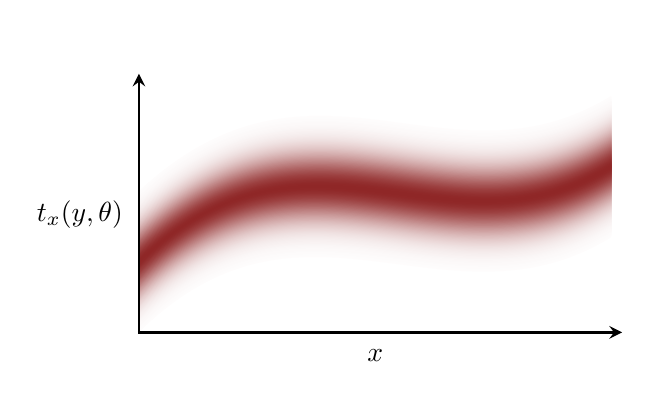
\begin{tikzpicture}[scale=0.3, thick]

  \foreach \i in {3, 2.95, ..., 0} {
    \pgfmathsetmacro{\prop}{100 * exp(-0.5 * \i * \i)};
    \colorlet{custom}{dark!\prop!white};
    \pgfmathsetmacro{\dy}{\i}
    \fill[color=custom] (-10, 3 + \dy) .. controls (-2.5, 9.9 + \dy) and (3, 2.75 + \dy) .. (10, 7.025 + \dy)
                         -- (10, 7.025 - \dy) .. controls (3, 2.75 - \dy)  and (-3, 9.9 - \dy) .. (-10, 3 - \dy);
  }

  %\draw[domain=-10:10, smooth, samples=150, line width=0.5, variable=\x, color=green] 
  %  plot ({\x},{mu(\x)});

  \node[] at (-12.5, 5) { $t_{x}(y, \theta)$ };

  \draw [->, >=stealth, line width=1] (-10.05, 0) -- +(20.5, 0);
  \draw [->, >=stealth, line width=1] (-10, -0.05) -- +(0, 11);
  \node[] at (0, -1) { $x$ };
  
  
  
\end{tikzpicture}

\end{document}  